\documentclass{beamer}

\setbeamercolor{framesubtitle}{fg=black}
\setbeamercolor{frametitle}{fg=white}
\setbeamercolor{navigation symbols}{fg=white, bg=white}
\setbeamercolor{section in toc}{fg=black}
\setbeamercolor{title}{fg=black}
\setbeamerfont{framesubtitle}{series=\bfseries, size=\large}
\setbeamerfont{frametitle}{series=\bfseries}
\setbeamerfont{institute}{size=\normalsize}
\setbeamerfont{section in toc}{series=\bfseries}
\setbeamerfont{subsection in toc}{series=\bfseries}
\setbeamerfont{title}{series=\bfseries}
\setbeamertemplate{frametitle}[default][right]
\setbeamertemplate{section in toc shaded}[default][50]
\setbeamertemplate{section in toc}[sections numbered]
\setbeamertemplate{sidebar right}{}
\setbeamertemplate{subsection in toc shaded}[default][50]
\setbeamertemplate{subsection in toc}[subsections numbered]

\addtobeamertemplate{footline}{%
    \hfill\usebeamertemplate***{navigation symbols}
    \hspace*{1em}\par\vspace{1pt}
}{}

\usepackage[UTF8]{ctex}
\usepackage[sort&compress]{natbib}
\usepackage{graphicx}
\usepackage{verbatim}
\usepackage{listings}


\AtBeginSection[]
{%
    \begin{frame}<beamer>
    \frametitle{目录}
    \tableofcontents[currentsection]
    \end{frame}
}

\AtBeginSubsection[]
{%
    \begin{frame}<beamer>
    \frametitle{目录}
    \tableofcontents[currentsection,currentsubsection]
    \end{frame}
}

\title{Tomcat 配置 性能调优与基准测试}
\author{author:xiaoyulong }
\institute{Aomi}
\date{\today}

\begin{document}

\usebackgroundtemplate{%
    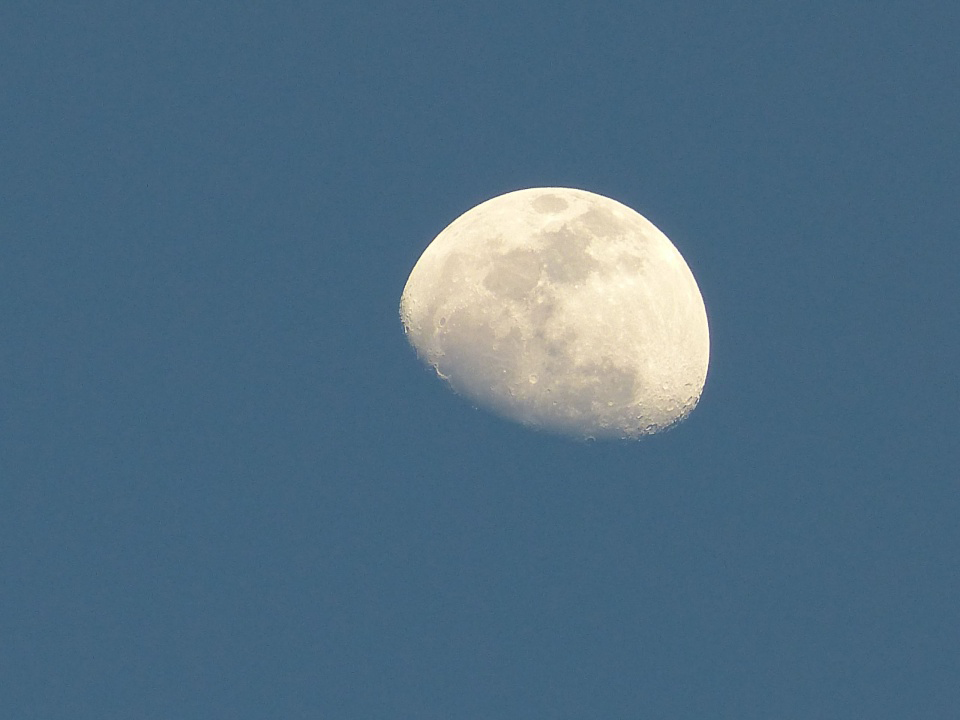
\includegraphics[width=\paperwidth,height=\paperheight]{img/title.png}
}

\frame{\titlepage}

\usebackgroundtemplate{%
    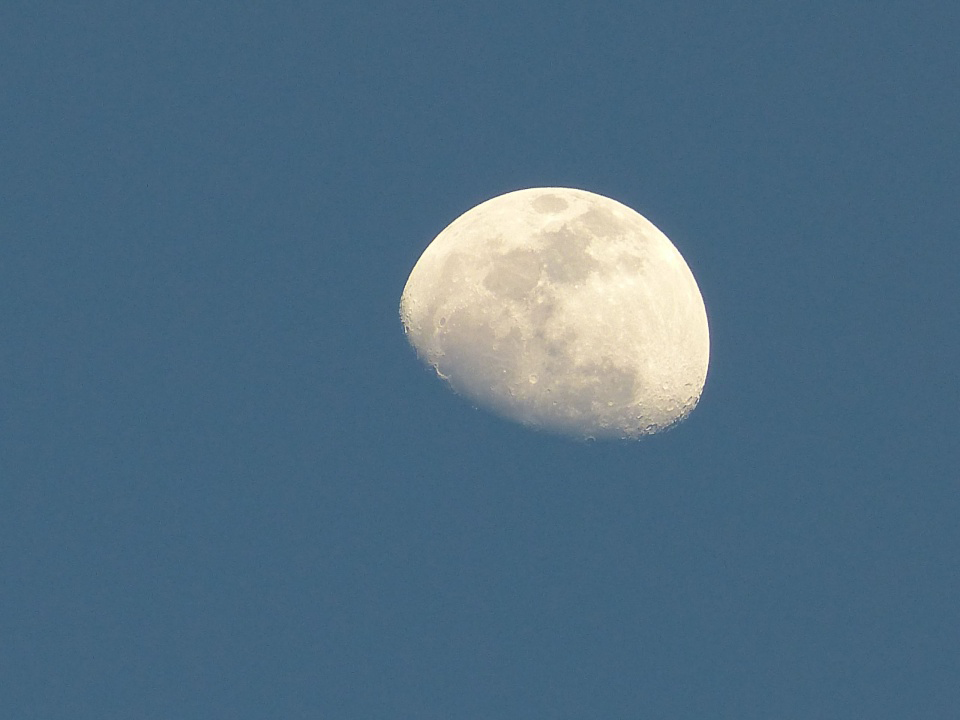
\includegraphics[width=\paperwidth,height=\paperheight]{img/content.png}
}

\begin{frame}
    \frametitle{目录}
    \tableofcontents[subsubsectionstyle=hide]
\end{frame}

\section{第一章节 Tomcat 配置}



\subsection{第一小节 TomCat 启动参数 }

\begin{frame}
    \frametitle{第一章节 Tomcat 配置}
    \framesubtitle{第一小节 TomCat 启动参数}
     \begin{itemize}
    	\item 参数配置
    	\item 参数解释
    \end{itemize}
\end{frame}

\begin{frame}
\frametitle{正标题}
   \centering
\begin{tabular}{|l|c|r|}
	\hline 
  \Huge	操作系统&  \Huge 默认GC&  \Huge 性能 \\
	\hline 
	JDK8 & G1非并发 &  GC \\
	\hline 
	JDK11 & G1并发 & GC \\
	\hline 
	openjdk8 & G1非并发& GC  \\
	\hline 
	openjdk11& G1并发 & GC \\
	\hline
\end{tabular}
\end{frame}


\subsection{第二小节 server.xml tomcat 配置参数}

\begin{frame}
    \frametitle{第一章节 Tomcat 配置}
    \framesubtitle{第二小节 server.xml tomcat 配置参数}
    
\end{frame}

\begin{frame}
\frametitle{JDK版本 与GC}
\centering
\begin{tabular}{|l|c|r|}
	\hline 
	\Huge	Connector&  \Huge 版本要求&  \Huge IO \\
	\hline 
	Http11Protocol & 7、8、9 & BIO \\
	\hline 
	Http11NioProtocol & 7、8、9 & NIO \\
	\hline 
	Http11Nio2Protocol & 8、9& NIO2  \\
	\hline 
	Http11AprProtocol& 7、8、9 & APR \\
	\hline
\end{tabular}
\end{frame}

\section{第二章节 基准测试}



\begin{frame}
\frametitle{Tomcat 基准性能}

\end{frame}


\section{参考文献}

\begin{frame}[allowframebreaks]
    \frametitle{参考文献}
    \small
    \bibliographystyle{plain}
    \bibliography{slide}
\end{frame}

\section*{}

\usebackgroundtemplate{%
    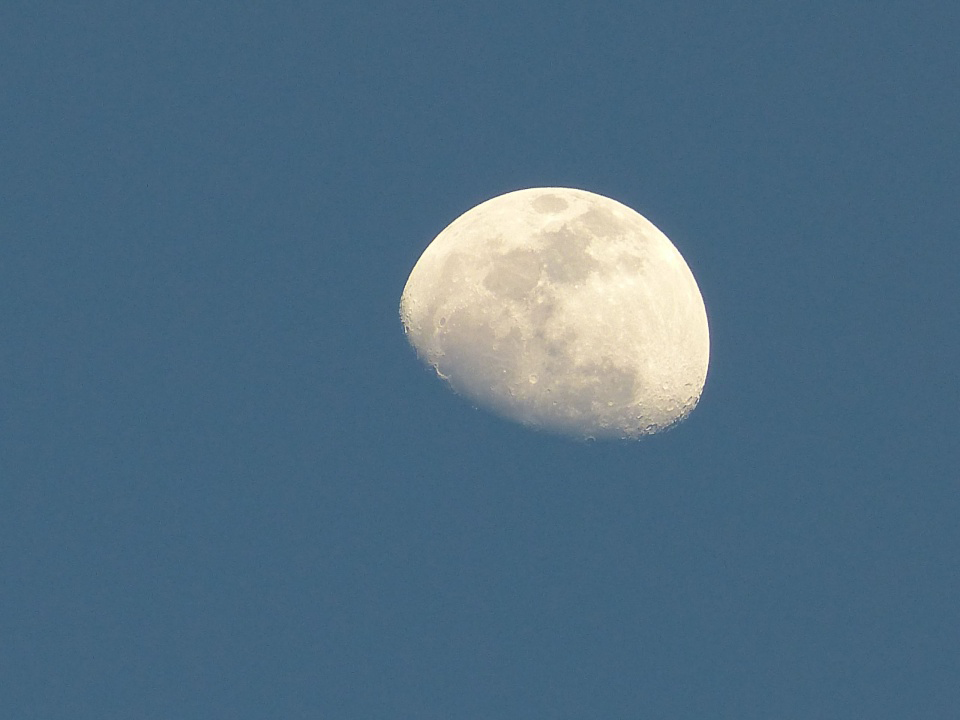
\includegraphics[width=\paperwidth,height=\paperheight]{img/title.png}
}

\begin{frame}
    \centering
   \Huge Q \& A
\end{frame}

\begin{frame}
\centering
\Huge Thank you !
\end{frame}

\end{document}
